%interaction with it, programs, geometry represenations, datastructures, formats etc., maybe even history if we're overkill
%\subsection{CAD in engineering}
Computer Aided Design (CAD) refers to the process of designing a product using a computer system. Before CAD applications were used, products were designed using a sketch board. It was a challenge to incorporate changes in the construction drafts as well as to keep documentations up to date; hence, it was no surprise that CAD systems spread rapidly across all design development branches. Computer aided design is now of irreplaceable use in architecture, mechanical, electrical and civil engineering.

Depending on the discipline, different requirements are set on the virtual model. One may imagine that in a civil engineering model of a building a 2D floor plan is often sufficient; however, in the design of a mechanical motor a 3D model is always necessary. Given these circumstances, various CAD software bundles evolved in the different disciplines with completely different modelling approaches. Besides the geometry representation additional parameters, such as material properties or manufacturing information, are stored. In order to move between different data structures standardized exchange interfaces are commonly used. 

This section presents the relevant geometrical and computational aspects of CAD for the project; for a more thorough introduction we refer to \cite{sarcarCAD}.

\subsection{Geometry representations}
In general, two different ways of describing a geometry are used in CAD systems: a \emph{constructive solid geometry} (CSG) or a \emph{boundary representation} (BREP). Other approaches, such as a complete voxelised geometry are not common due to extensive memory consumption.
\subsubsection{Constructive solid geometry}
\begin{figure}
\centering
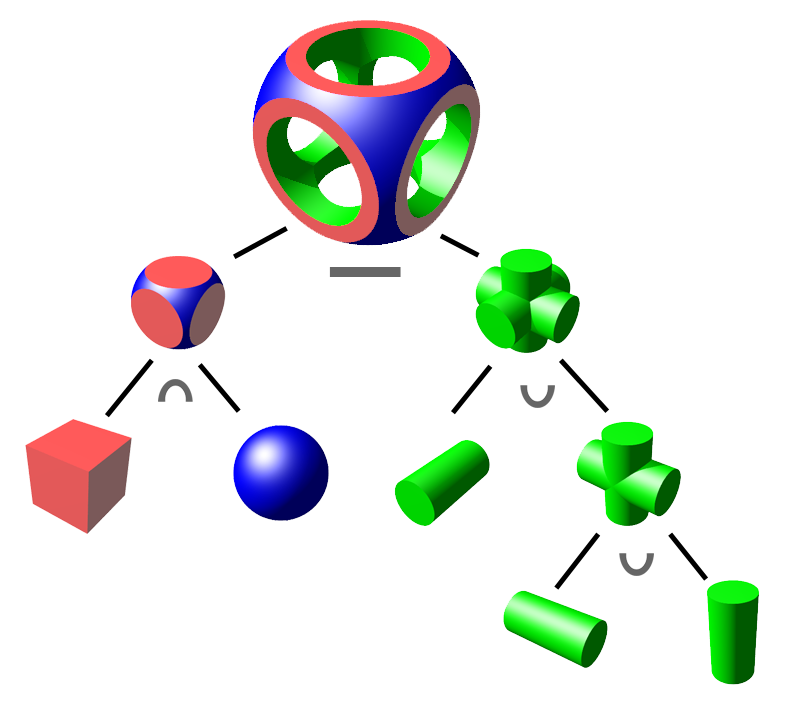
\includegraphics[width=0.5\textwidth]{Pictures/Csg_tree.png}
\caption{CSG object tree. The picture shows the construction of a complex object from a cube, a sphere, and a set of cylinders. Figure taken from \cite{WikipediaCSG}}.
\label{fig:csg_tree}
\end{figure}
One way of representing a geometry in CAD is the approach of \emph{constructive solid geometry}. The basic idea is to start from a set of primitives, e.g. spheres, cylinders and/or cubes. Basic Boolean operations link these primitives towards a complex geometry, as illustrated in \autoref{fig:csg_tree}.

Key advantages of this format is the precise representation using very little storage memory. However, not all desired forms can be represented by CSG and hence, a second type of geometry description is needed. 
\subsubsection{Boundary representation}
A different kind of modelling approach is the so-called \emph{boundary representation}. Instead of storing the geometry information as geometrical objects, BREP formats only save the boundary surface of the body. The interior is assumed to be uniformly filled. Especially in complex geometries, this approach simplifies the model to such an extent, that the amount of data becomes much easier to handle. Surfaces can then be for example stored as a set of triangles (as in STL files, see \autoref{subsub:STL} below) or in NURBS patches (see \autoref{sec:NURBS}).
Furthermore, holes in the body are made possible by saving the surface normal of the respective boundary. 

By the boundary representation arbitrary geometries can be created. While the data sizes are commonly larger than in CSG representation, BREP files are usually easier to work with. One also has to keep in mind, that non-physical geometries can result from BREP formats through a not closed surface.
\subsection{Data exchange interfaces}
CAD software programs usually use their own data formats; in order to exchange models standardized interface formats have been developed. Geometric models are compressed to certain geometry descriptions; transferring additional information, such as material properties or manufacturing information, is in general a difficult task and in some exchange file formats even prohibited. A few common exchange file types are described below, as also compared in \cite{STL}.
\subsubsection{STL file format} \label{subsub:STL}
The STL (from \emph{ST}ereo\emph{L}ithography) file format describes the model only by its boundary and is thus a BREP format. The idea behind it files is simple. The geometric model is discretized into a cloud of points, where sets of three vertices form a triangle; hence, a connected surface of triangles emerges which describes the geometry. The procedure is shown in \autoref{fig:STL} for a two dimensional circle.  
\begin{figure}
\centering
   \scalebox{0.4}{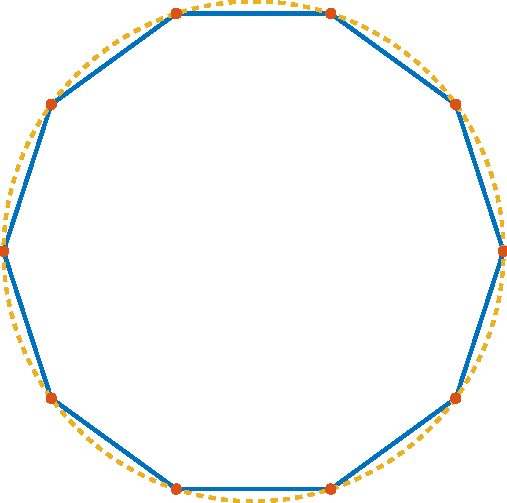
\includegraphics{Pictures/STL.pdf}}\\
   \caption{STL discretization for a circle, self-made in MATLAB. Note that the circle cannot be exactly represented by the vertices and edges.}
   \label{fig:STL}
\end{figure}
The aforementioned triangles boil down to lines in two dimensions. The advantages and disadvantages of this approach become clear: It can be applied to an arbitrary geometry, but accuracy causes difficulties. In order to transfer high precision geometries many vertices are necessary, resulting in big files. Still, as can be seen in the figure, a perfect circle can never be represented. 

ASCII STL files begin with a name and the data on the triangles is constructed as follows: 
\begin{itemize}
\item a facet normal pointing outward
\item a sequence of vertex coordinates
\end{itemize}
As this is the only information provided, no additional data such as material properties are transferred through STL files, reducing file size but also range of usage.
\subsubsection{STEP file format}
To overcome issues of insufficient precision also more elaborate exchange formats exist; these save e.g. a circle as a parameter where no discretization step is involved. Also, the possibility of passing additional parameter information (e.g. density, manufacturing information) is required by certain users. Popular file types that offer these two functionalities are STEP and IGES files. 

The STEP file format is a newly developed CAD data exchange standard and documented in the ISO 10303 norm. On the contrary to STL files it uses a combination of CSG and BREP to store the geometry. Additional information (e.g. density) are passed through attribute sets that are stored besides geometry instances (e.g. a circle). A key disadvantage, however, is that STEP files carry much redundant information \cite{STL}.
\subsubsection{IGES file format}
 The Initial Graphics Exchange Specification (IGES) is an American 
National Standard since 1981 to exchange graphics information. Similar to the STEP format it uses a combination of CSG and BREP for the geometry representation. Instead of storing a set of manufacturing information as done in the STEP file, the IGES is build only to exchange graphics information. For example, the step file transfers a physical density information; in the IGES format the only additional parameter store node coloring information. Consequentially, IGES file sizes are significantly smaller compared to the STEP file format \cite{STL}.

The IGES file format contains five different sections: a \emph{Start}, \emph{Global}, \emph{Directory Entry}, \emph{Parameter Data} and \emph{Terminate} section. The \emph{Start} and \emph{Global} section are used for naming and part information. In the \emph{Directory Entry} section additional information like the node color is saved. The \emph{Parameter Data} section is used for storing the coordinate points; the \emph{Terminate} section signals the end of the file \cite{sarcarCAD}.
